\documentclass{article}

\usepackage{ctex}
\usepackage[top=0.7in,bottom=0.7in,left=0.5in,right=0.5in]{geometry}
\usepackage{array}
\usepackage{multirow}
\usepackage{graphicx}
\usepackage{subfigure}
\usepackage{fancyhdr}
\usepackage{lastpage}
\usepackage{extramarks}
\usepackage{amsmath}
\usepackage{listings}
\usepackage{fontspec}
\usepackage[colorlinks,
            linkcolor=black,
            anchorcolor=black,
            citecolor=black
            ]{hyperref}
\newfontfamily\consolas{Consolas}
\usepackage{xcolor} % 定制颜色
\definecolor{mygreen}{rgb}{0,0.6,0}
\definecolor{mygray}{rgb}{0.5,0.5,0.5}
\definecolor{mymauve}{rgb}{0.58,0,0.82}
\lstset{ %
backgroundcolor=\color{white},      % choose the background color
basicstyle=\footnotesize\ttfamily,  % size of fonts used for the code
columns=fullflexible,
tabsize=4,
breaklines=true,               % automatic line breaking only at whitespace
captionpos=b,                  % sets the caption-position to bottom
commentstyle=\color{mygreen},  % comment style
escapeinside={\%*}{*)},        % if you want to add LaTeX within your code
keywordstyle=\color{blue},     % keyword style
stringstyle=\color{mymauve}\ttfamily,  % string literal style
frame=single,
rulesepcolor=\color{red!20!green!20!blue!20},
% identifierstyle=\color{red},
language=c++,
}

\newcommand{\hmwkTitle}{用先序遍历建立二叉树\ 实验报告}
\newcommand{\hmwkClass}{数据结构}
\newcommand{\hmwkClassInstructor}{}
\newcommand{\hmwkAuthorName}{毛子恒\ 李臻\ 张梓靖}

\pagestyle{fancy}
\lhead{\hmwkAuthorName}
\chead{\hmwkClass\ : \hmwkTitle}
\rhead{\firstxmark}
\lfoot{\lastxmark}
\cfoot{\thepage}
\renewcommand\headrulewidth{0.4pt}
\renewcommand\footrulewidth{0.4pt}

\title{\hmwkClass\ :\hmwkTitle}
\author{\hmwkAuthorName}

\setcounter{tocdepth}{1}

\begin{document}

\maketitle

\section*{小组成员}

\setlength{\tabcolsep}{9mm}
{
    \begin{table}[htbp]
        \centering
        \begin{tabular}{llll}
            班级:2019211309 & 姓名:毛子恒 & 学号:2019211397 & 分工:代码\ 文档   \\

            班级:2019211310 & 姓名:李臻   & 学号:2019211458 & 分工:测试\ 文档   \\

            班级:2019211308 & 姓名:张梓靖 & 学号:2019211379 & 分工:可视化\ 文档 \\
        \end{tabular}
    \end{table}
}

\tableofcontents
\newpage

\section{需求分析}

\subsection{题目描述}

按照先序遍历输入一个二叉树,建立二叉树,输出该二叉树的各种表示形式。

\subsection{输入描述}

程序从标准输入中读入数据。

输入的第一行为一个字符串,表示二叉树按先序遍历所得的序列。用*字符代表空树。

之后按照提示输入选项,参考5\ 用户使用说明。

\subsection{输出描述}

程序向标准输出中打印结果。

若选择输出图形化表示,则打印若干行,表示二叉树的图形。

若选择输出遍历结果,则打印一行,表示二叉树某种遍历的结果。

若程序出现运行时错误,则没有输出。

\subsection{样例输入输出}

\subsubsection{样例输入输出1}

见图1。

\begin{figure}[htbp]

    \centering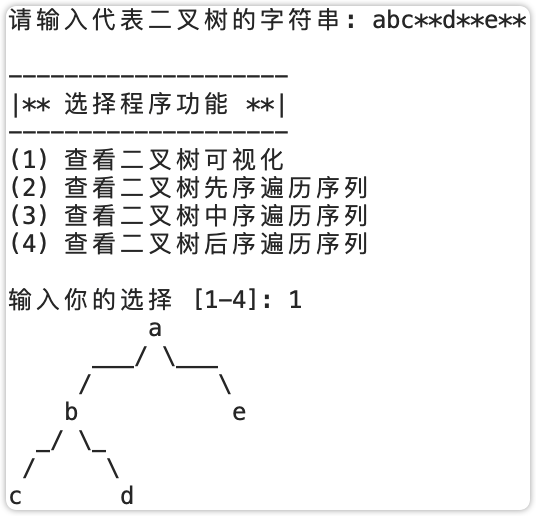
\includegraphics[width=0.4\textwidth]{./Images/sample1.png}

    \caption{样例输入输出1}

\end{figure}

\subsubsection{样例输入输出2}

见图2。

\begin{figure}[htbp]

    \centering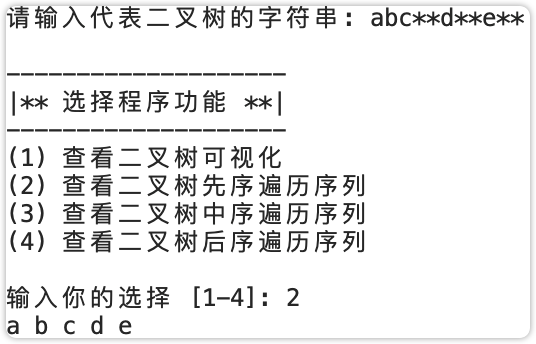
\includegraphics[width=0.4\textwidth]{./Images/sample2.png}

    \caption{样例输入输出2}

\end{figure}

\subsubsection{样例输入输出3}

见图3。

\begin{figure}[htbp]

    \centering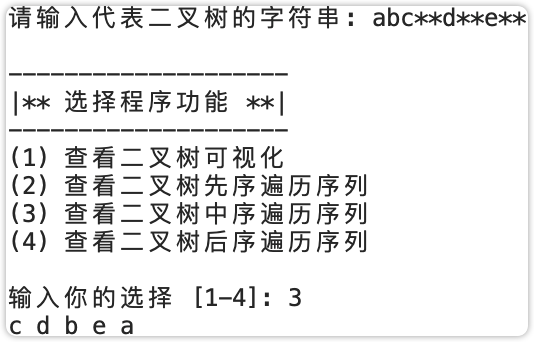
\includegraphics[width=0.4\textwidth]{./Images/sample3.png}

    \caption{样例输入输出3}

\end{figure}

\subsubsection{样例输入输出4}

见图4。

\begin{figure}[htbp]

    \centering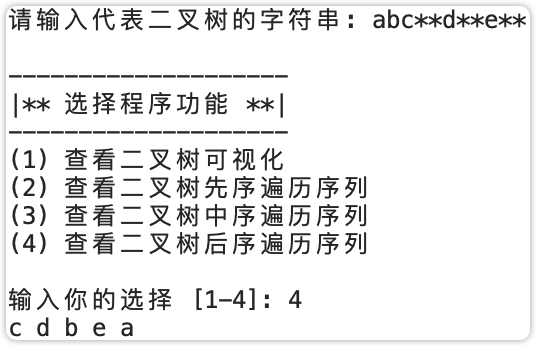
\includegraphics[width=0.4\textwidth]{./Images/sample4.png}

    \caption{样例输入输出4}

\end{figure}

\subsection{程序功能}

程序通过先序遍历序列生成二叉树,根据选项打印二叉树的图形或者某种遍历结果。

\section{概要设计}

\subsection{问题解决的思路}

使用二叉链表存储二叉树,并且设计输出二叉树图形的算法、二叉树的先序、中序、后序遍历算法。

\subsection{二叉树的定义}

\begin{lstlisting}[language={C},
    numbers=left,
    numberstyle=\tiny\consolas,
    basicstyle=\small\consolas]
//数据对象
typedef struct node
{
    char data;
    struct node * lc, * rc; // 左右孩子指针
    int pos; // 记录结点位置,用于输出二叉树图形
} Node;

/*
 * 操作:建二叉树
 * 前件:标准输入流中为一个字符串,代表二叉树
 * 后件:建立一个二叉树,返回指向该二叉树根节点的指针
 */
Node * buildTree();

/*
 * 操作:先序遍历
 * 前件:point指向一个二叉树的根节点
 * 后件:向标准输出中打印二叉树的先序遍历序列
 */
void preOrderTraverse(Node * point);

/*
 * 操作:中序遍历
 * 前件:point指向一个二叉树的根节点
 * 后件:向标准输出中打印二叉树的中序遍历序列
 */
void inOrderTraverse(Node * point);

/*
 * 操作:后序遍历
 * 前件:point指向一个二叉树的根节点
 * 后件:向标准输出中打印二叉树的后序遍历序列
 */
void postOrderTraverse(Node * point);

/*
 * 操作:输出二叉树图形
 * 前件:point指向一个二叉树的根节点
 * 后件:向标准输出中打印二叉树的图形
 */
void printGraph(Node * point);

/*
 * 操作:释放二叉树空间
 * 前件:point指向一个二叉树的根节点
 * 后件:释放该二叉树占用的空间
 */
void destroyTree(Node * point);
\end{lstlisting}

\subsection{主程序的流程}

\begin{enumerate}
    \item 输入字符串
    \item 建二叉树
    \item 依照输入的选项打印相应的结果
    \item 询问是否要继续选择其他选项,如果继续,回到第三步
    \item 释放空间
\end{enumerate}

\subsection{各程序模块之间的层次关系}

程序模块层次关系图如图5。

\begin{figure}[htbp]

    \centering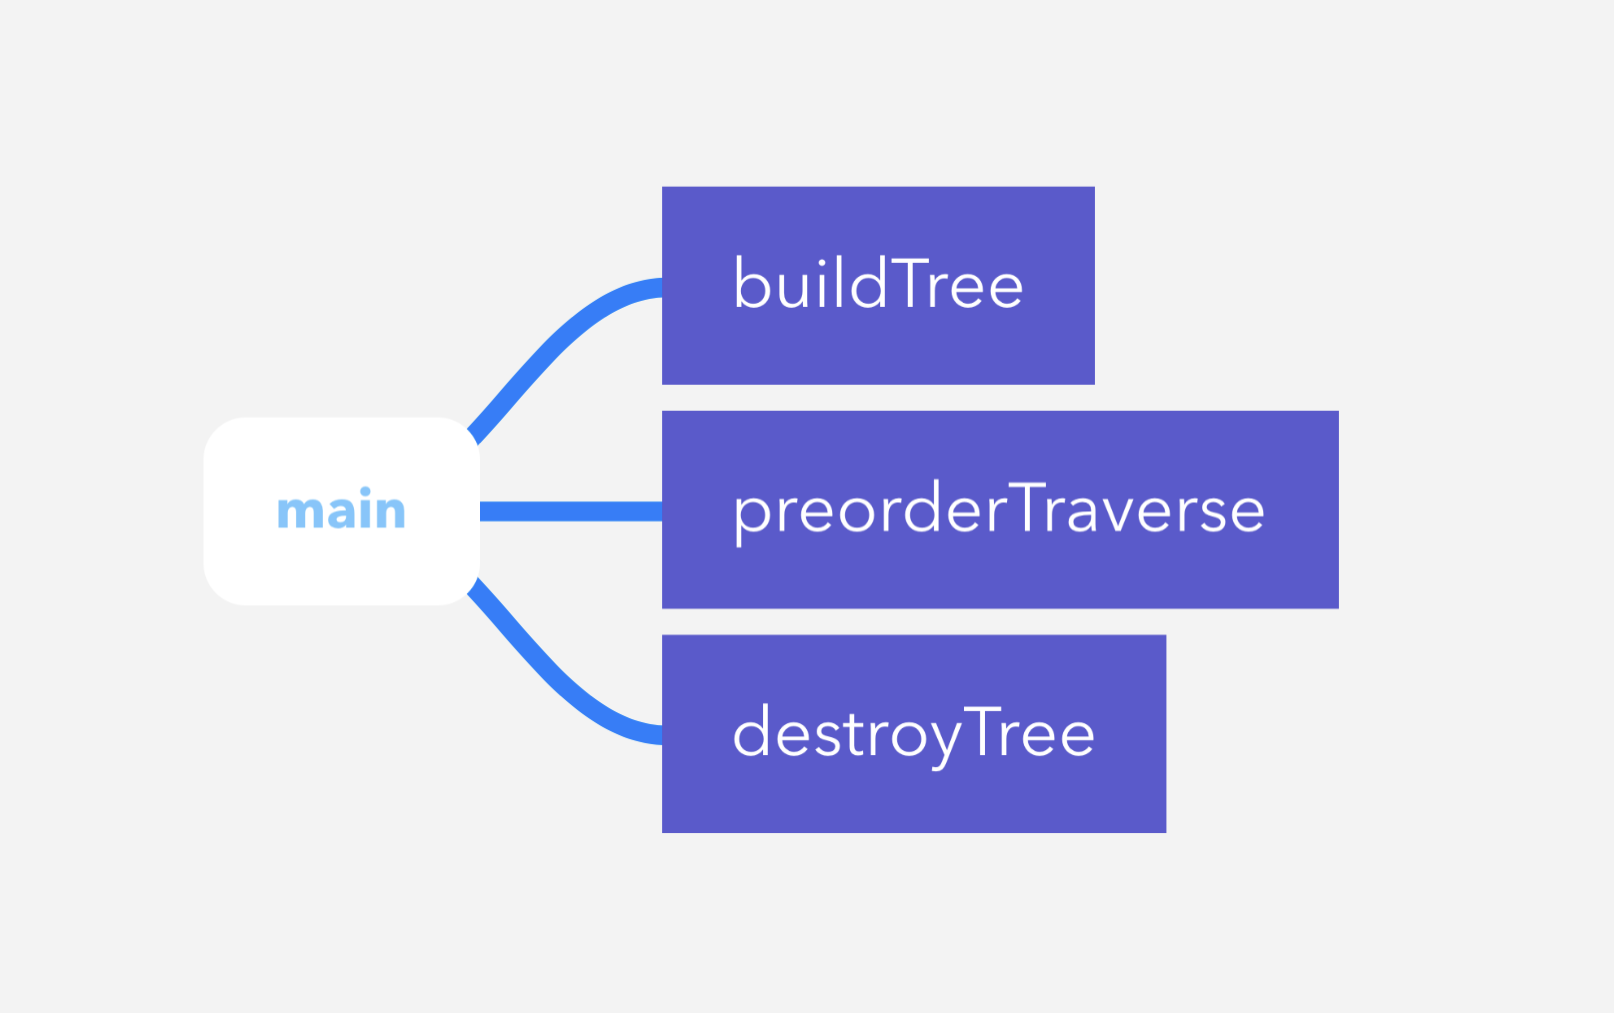
\includegraphics[width=0.4\textwidth]{./Images/pic4_1_1.png}

    \caption{程序模块层次关系}

\end{figure}

\section{详细设计}

\subsection{二叉树的实现}

二叉树的设计中基本操作的伪代码算法如下:

\begin{lstlisting}[language={C},
    numbers=left,
    numberstyle=\tiny\consolas,
    basicstyle=\small\consolas]
// 生成二叉树
// 建二叉树
Node * buildTree()
{
    读入字符ch
    if (ch为'*')
        返回空指针
    创建新节点,并用point指针指向它,如果内存分配失败,异常退出
    point->data <- ch
    分别建point的左子树和右子树,并且更新lc和rc指针
    计算二叉树的图形中该点的位置
    每两个叶结点之间需要空出8个字符的宽度
    度为1的结点的空子树也要空出8个字符的宽度
    非叶结点的位置为两个孩子结点位置的平均值
    返回point
}

// 先序遍历
void preOrderTraverse(Node * point)
{
    输出point->data
    if (point的左子树不为空)
        preOrderTraverse(point->lc);
    if (point的右子树不为空)
        preOrderTraverse(point->rc);
}

// 中序遍历
void inOrderTraverse(Node * point)
{
    if (point的左子树不为空)
        inOrderTraverse(point->lc);
    输出point->data
    if (point的右子树不为空)
        inOrderTraverse(point->rc);
}

// 后序遍历
void postOrderTraverse(Node * point)
{
    if (point的左子树不为空)
        postOrderTraverse(point->lc);
    if (point的右子树不为空)
        postOrderTraverse(point->rc);
    输出point->data
}

// 输出二叉树图形
void printGraph(Node * point)
{
    定义队列和队列的头指针、尾指针
    初始化队列中的唯一一个元素为根结点
    while (h <= t)
    {
        每层的图形第一行:输出该层结点的字符数据,并用空格补齐间距
        换行
        每层图形的第二行:输出根节点下的斜杠和反斜杠,以及代表边下划线,并用空格补齐间距
        换行
        每层图形的第三行:输出孩子结点上的斜杠和反斜杠,孩子结点入队,并用空格补齐间距
        换行
    }
}

// 释放二叉树空间
void destroyTree(Node * point)
{
    if (point的左子树不为空)
        destroyTree(point->lc);
    if (point的右子树不为空)
        destroyTree(point->rc);
    释放point指针
}
\end{lstlisting}

\subsection{函数的调用关系图}

函数调用关系图如图6。

\begin{figure}[htbp]

    \centering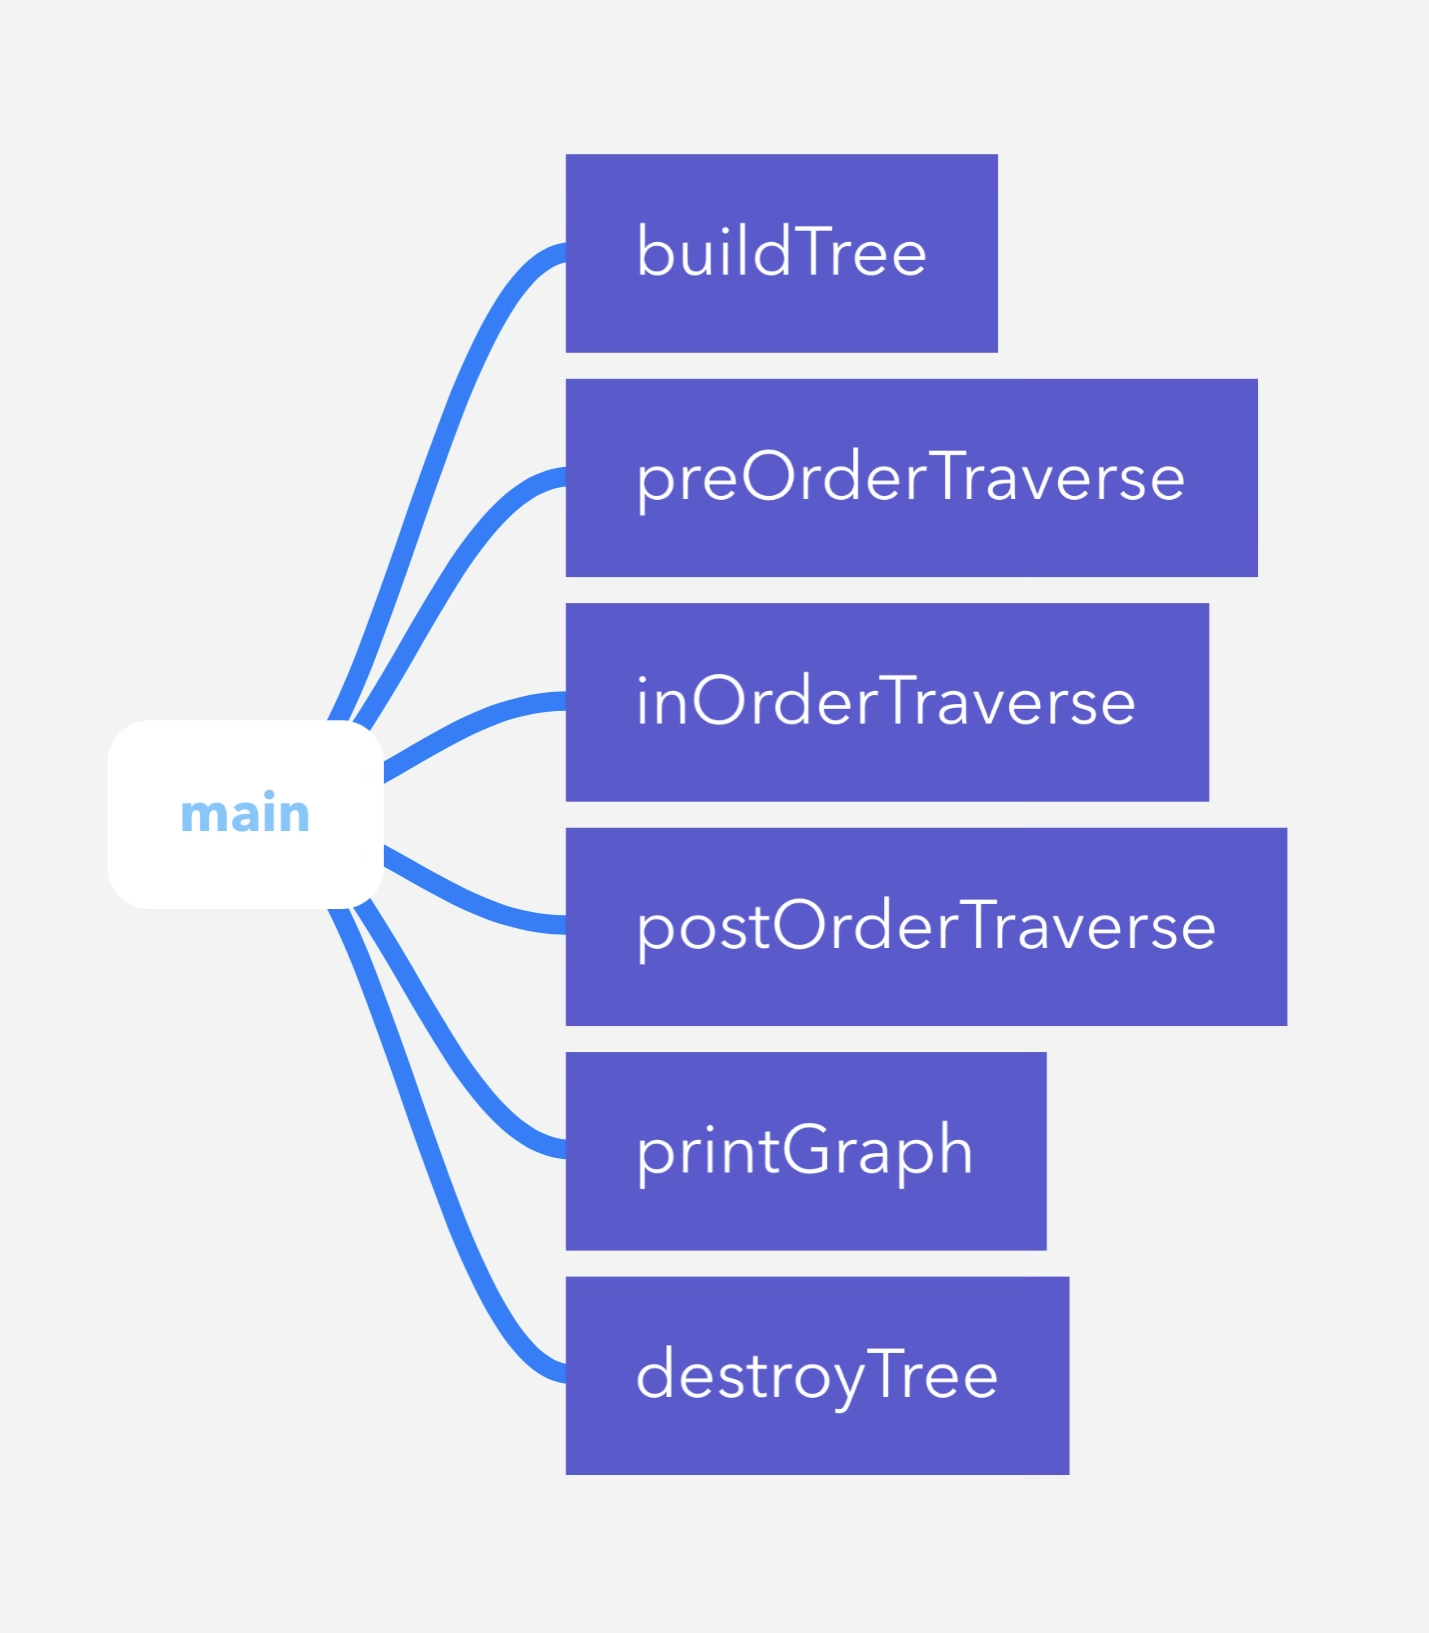
\includegraphics[width=0.4\textwidth]{./Images/pic4_1_2.png}

    \caption{函数调用关系图}

\end{figure}

\section{调试分析报告}

\subsection{调试过程中遇到的问题和思考}

在建树和遍历的过程中没有遇到太大问题,主要在输出二叉树的图形部分遇到比较大的困难。

最后决定采用两种实现方式,实现细节在4.2节和7节分别讨论。

\subsection{设计实现的回顾讨论}

在C实现的图形化当中,给每个叶结点和度数为1的结点的空子树留下长度为8的空格。通过'/'(斜杠),'$\backslash$'(反斜杠),'\_'(下划线)符号来表示二叉树的边。

由于需要兼顾时间复杂度和编程复杂度,在树中存在较多的链时会略微缺少可读性。

\subsection{算法复杂度分析}

printGraph函数的时间复杂度为$O(n^2)$。

其余函数的复杂度为$O(n)$。

主函数的时间复杂度为$O(1)$,整体时间复杂度为$O(n^2)$。

整体空间复杂度为$O(n)$。

\section{用户使用说明}

使用gcc编译生成可执行文件。

\begin{lstlisting}[language={bash},
    basicstyle=\small\consolas]
gcc -o main -std=c11 main.c binarytree.c
\end{lstlisting}

执行可执行文件:

\begin{lstlisting}[language={bash},
    basicstyle=\small\consolas]
./main
\end{lstlisting}

在Windows cmd下:

\begin{lstlisting}[language={bash},
    basicstyle=\small\consolas]
main
\end{lstlisting}

之后通过标准输入输入数据,首先按照提示输入1.2节描述的字符串,之后标准输出中会打印提示信息,根据提示信息
选择相应的选项(数字1$\sim$4),打印完成后根据提示,如果输入字符c则继续选择选项,输入字符q则退出程序。

如果输入合法并且程序正常运行结束,主函数返回值为0。

\section{测试结果}

测试环节分为两个步骤。

\subsection{测试第一部分}

对1.4节给出的样例进行测试。

\subsection{测试第二部分}

测试边界条件。

见图7。

\begin{figure}[htbp]

    \centering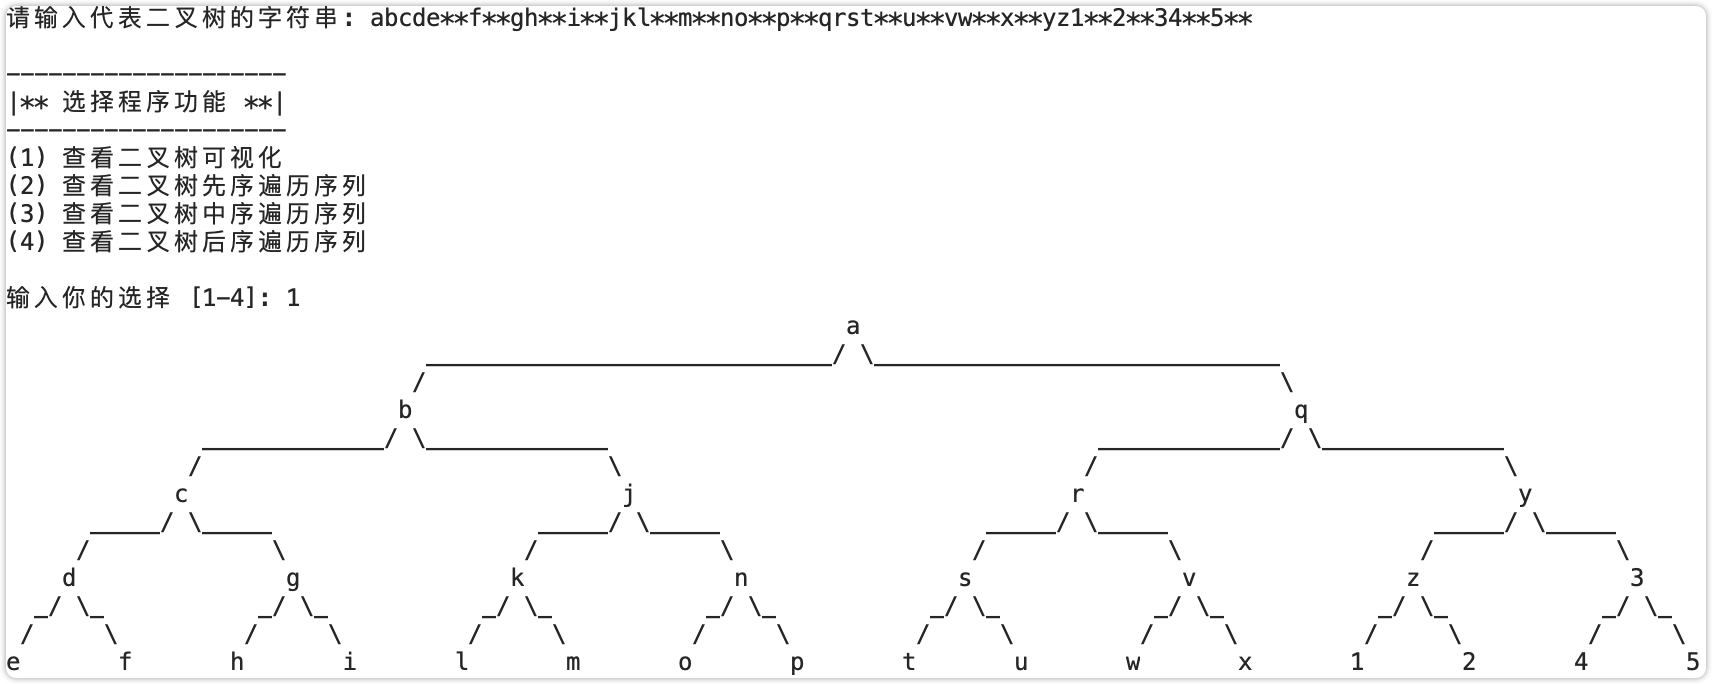
\includegraphics[width=0.95\textwidth]{./Images/sample5.png}

    \centering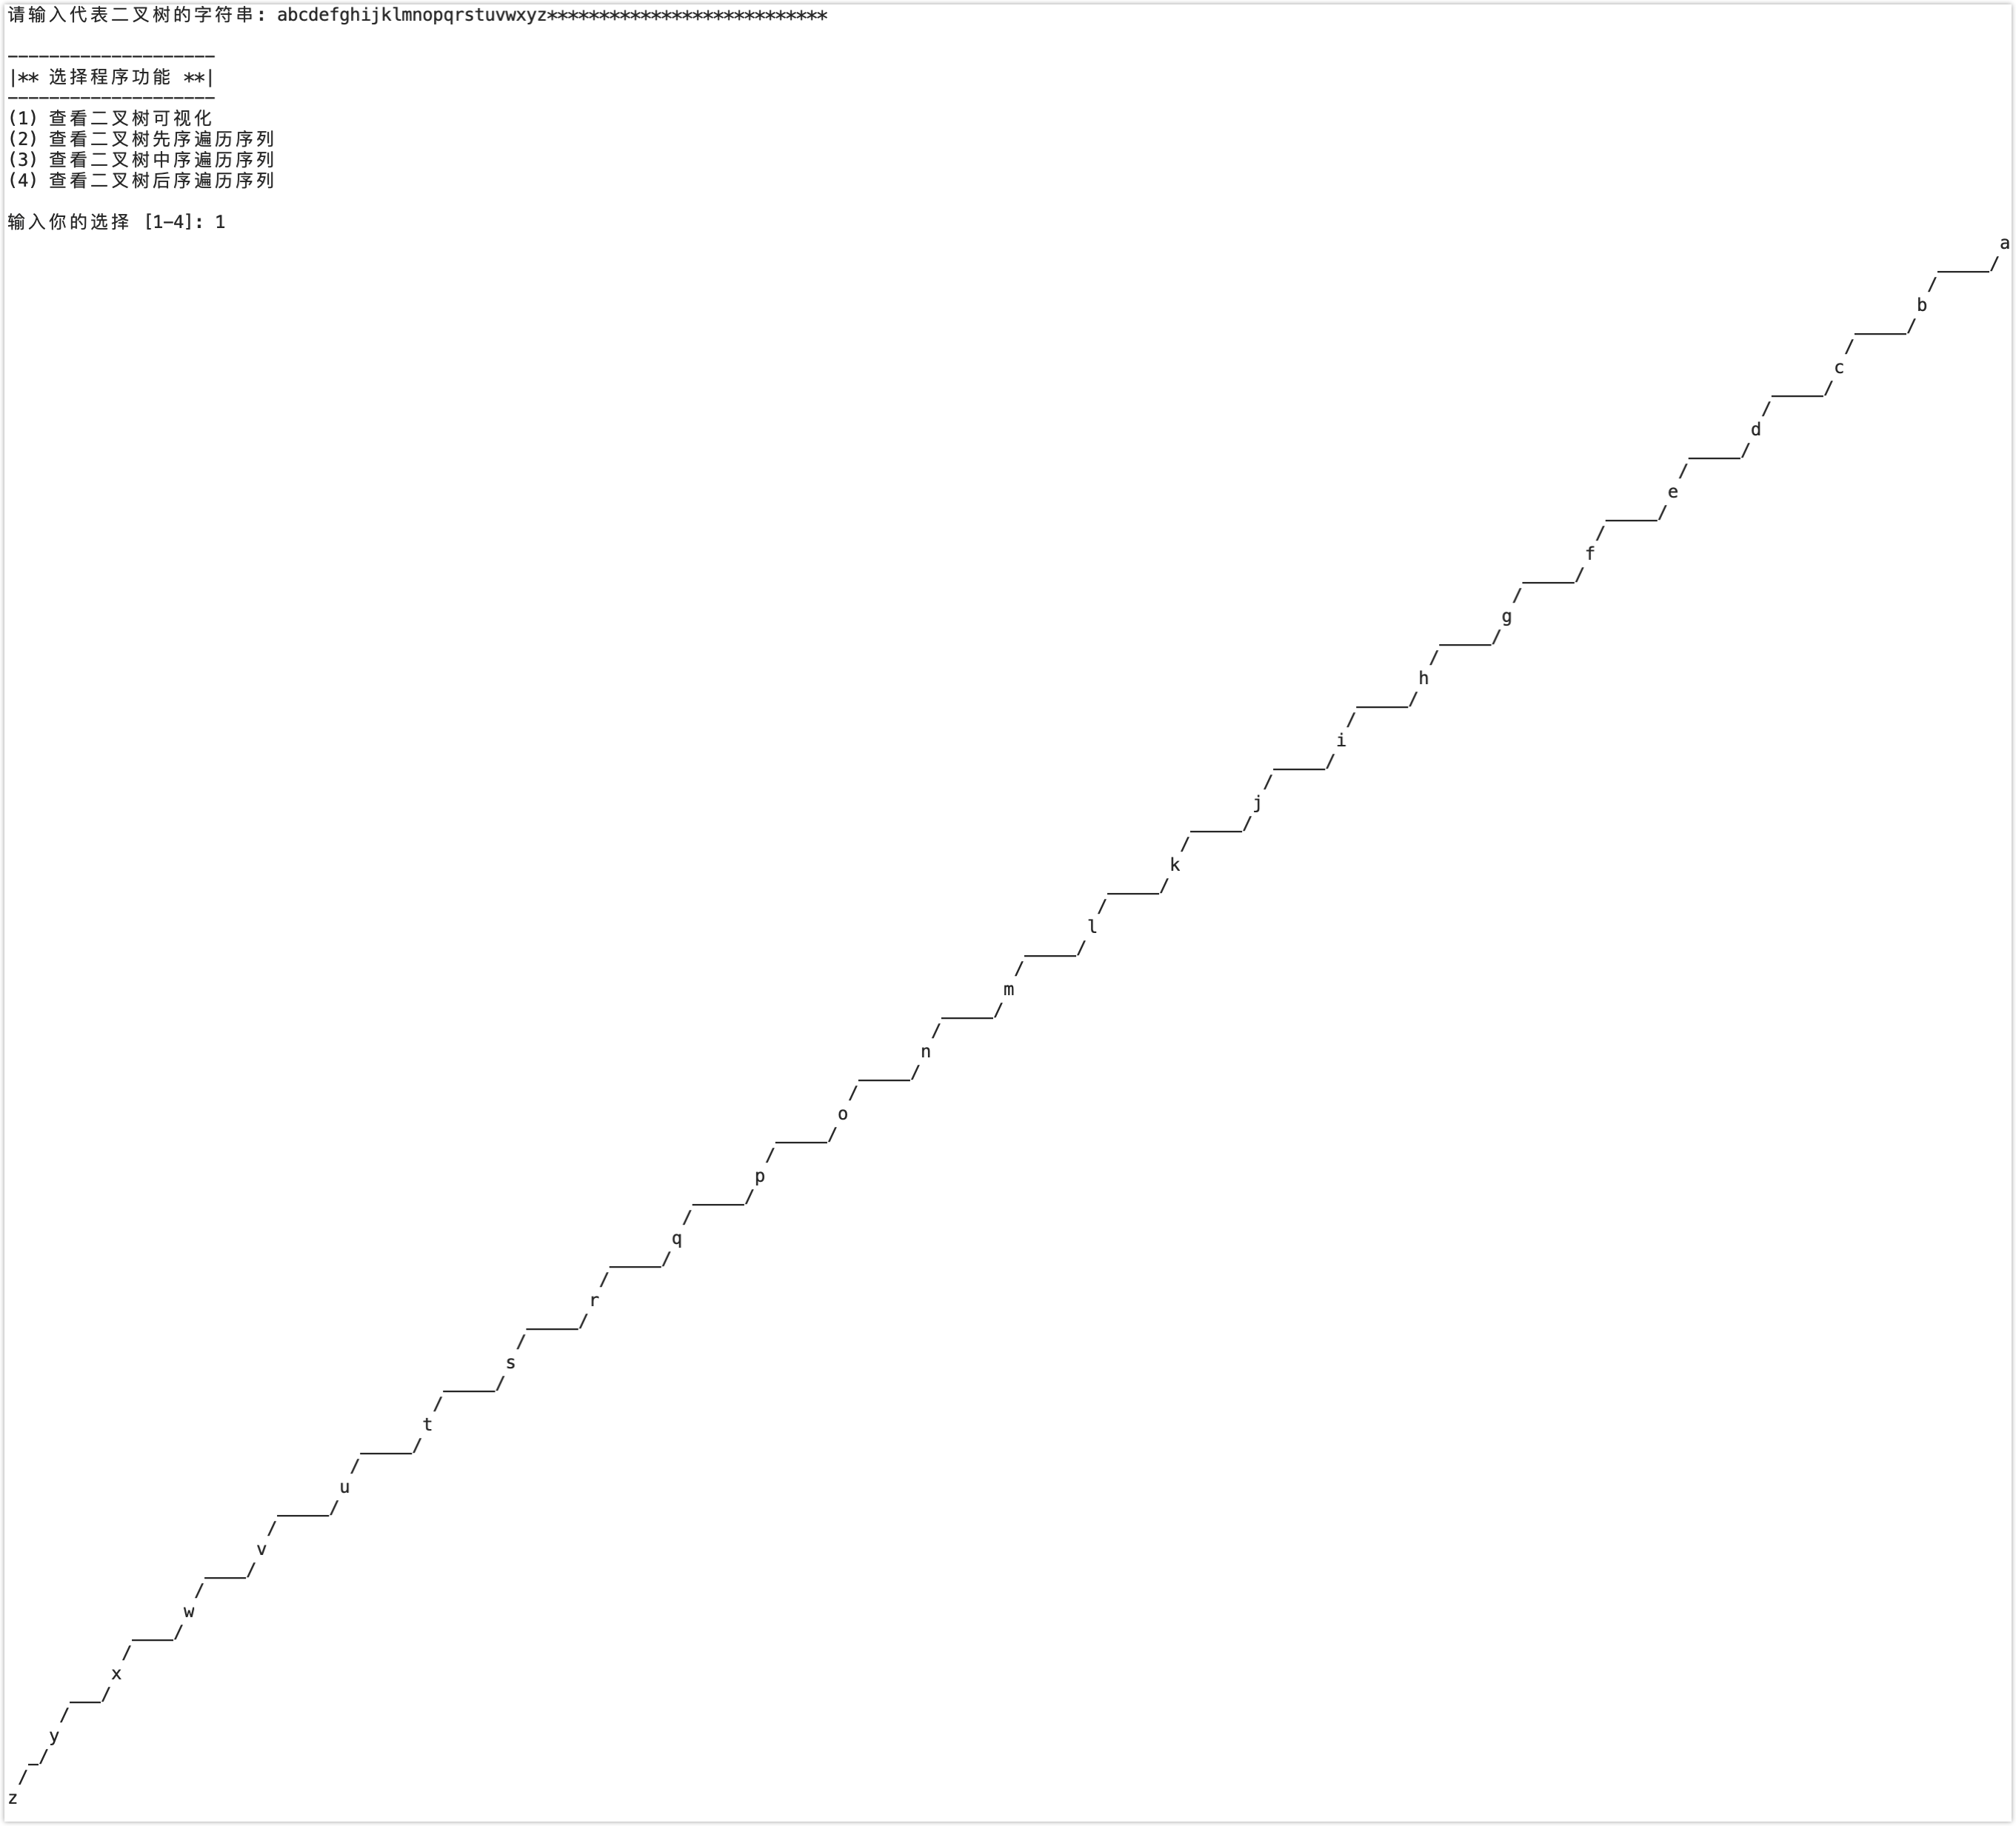
\includegraphics[width=0.95\textwidth]{./Images/sample6.png}

    \caption{边界测试}

\end{figure}

\section{可视化}

使用JavaScript实现二叉树的构建,调用d3.js库实现可视化。

\subsection{用户使用说明}

使用现代浏览器打开Visualization/index.html,输入字符串,即可看到可视化结果。

\subsection{示例}

见图8。

\begin{figure}[htbp]
    
    \centering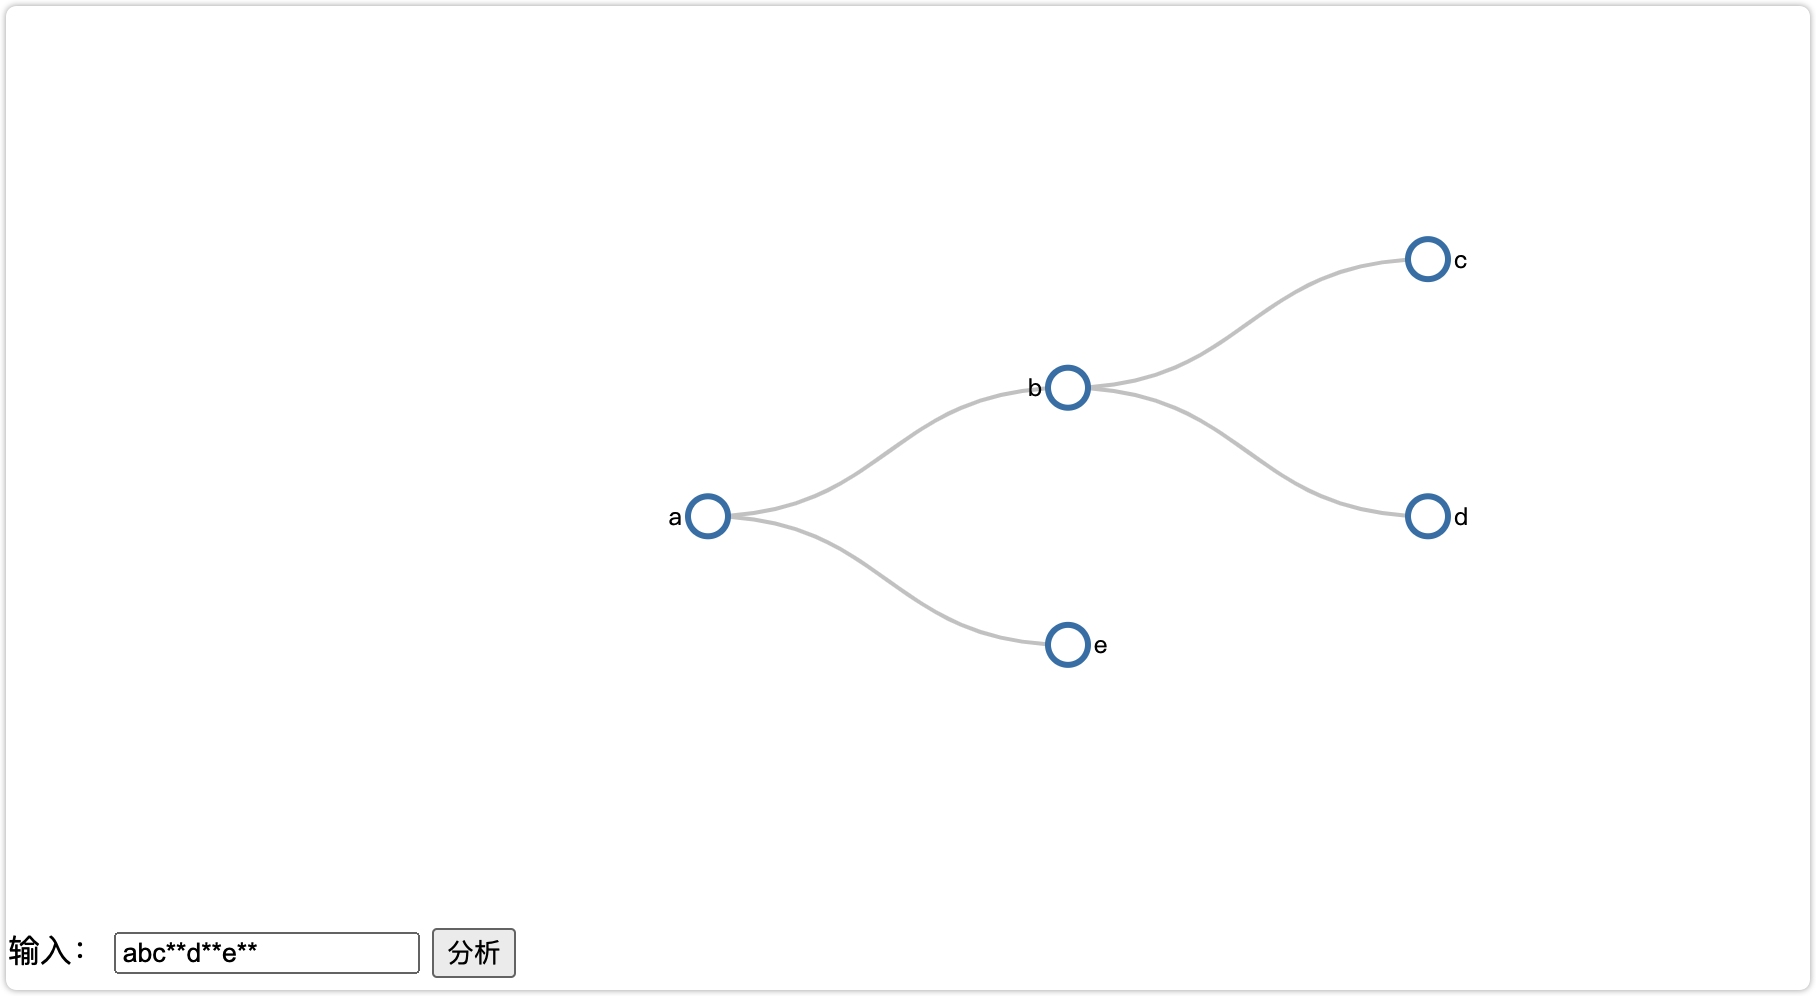
\includegraphics[width=0.9\textwidth]{./Images/pic4_1_3.png}
    
    \caption{可视化示例}
    
\end{figure}

\end{document}
